\chapter{hydrogen atom solutions}
\begin{abox}
	Practice set 1 solutions
	\end{abox}
\begin{enumerate}
\begin{minipage}{\textwidth}
	\item The energy levels of the non-relativistic electron in a hydrogen atom (i.e. in a Coulomb potential $V(r) \propto-1 / r$ ) are given by $E_{n l m} \propto-1 / n^{2}$, where $n$ is the principal quantum number, and the corresponding wave functions are given by $\psi_{n l m}$, where $l$ is the orbital angular momentum quantum number and $m$ is the magnetic quantum number. The spin of the electron is not considered. Which of the following is a correct statement?
	\exyear{NET JUNE 2011}
\end{minipage}
\begin{tasks}(1)
	\task[\textbf{A.}] There are exactly $(2 l+1)$ different wave functions $\psi_{n l m}$, for each $E_{n l m}$.
	\task[\textbf{B.}]There are $l(l+1)$ different wave functions $\psi_{n l m}$, for each $E_{n l m}$.
	\task[\textbf{C.}] $E_{n l m}$ does not depend on $l$ and $m$ for the Coulomb potential.
	\task[\textbf{D.}]There is a unique wave function $\psi_{n l m}$ for each $E_{n l m}$.
\end{tasks}
\begin{answer}
	The correct option is \textbf{(c)}
\end{answer}
\begin{minipage}{\textwidth}
	\item Let $\psi_{n l m_{l}}$ denote the eigenfunctions of a Hamiltonian for a spherically symmetric potential $V(r)$. The wavefunction $\psi=\frac{1}{4}\left[\psi_{210}+\sqrt{5} \psi_{21-1}+\sqrt{10} \psi_{211}\right]$ is an eigenfunction only of
	\exyear{NET JUNE 2012}
\end{minipage}
\begin{tasks}(2)
	\task[\textbf{A.}] $H, L^{2}$ and $L_{2}$
	\task[\textbf{B.}]$H$ and $L_{z}$
	\task[\textbf{C.}]$H$ and $L^{2}$
	\task[\textbf{D.}]$L^{2}$ and $L_{z}$
\end{tasks}
\begin{answer}
	$H \psi=E_{n} \psi$\\
	$L^{2} \psi=l(l+1) \hbar^{2} \psi$ and $L_{2} \psi \neq m \hbar \psi$.\\
	The correct option is \textbf{c}	
\end{answer}
\begin{minipage}{\textwidth}
	\item The wave function of a state of the Hydrogen atom is given by,
	$$
	\psi=\psi_{200}+2 \psi_{211}+3 \psi_{210}+\sqrt{2} \psi_{21-1}
	$$
	where $\psi_{n l m}$ is the normalized eigen function of the state with quantum numbers $n, l, m$ in the usual notation. The expectation value of $L_{z}$ in the state $\psi$ is
	\exyear{NET DEC 2012}
\end{minipage}
\begin{tasks}(2)
	\task[\textbf{A.}] $\frac{15 \hbar}{6}$
	\task[\textbf{B.}]$\frac{11 \hbar}{6}$
	\task[\textbf{C.}]$\frac{3 \hbar}{8}$
	\task[\textbf{D.}]$\frac{\hbar}{8}$
\end{tasks}
\begin{answer}
	Firstly normalize $\psi, \psi=\frac{1}{\sqrt{16}} \psi_{200}+\frac{2}{\sqrt{16}} \psi_{211}+\frac{3}{\sqrt{16}} \psi_{210}+\frac{\sqrt{2}}{\sqrt{16}} \psi_{21-1}$ \\
	$P(0 \hbar)=\frac{1}{16}+\frac{9}{16}=\frac{10}{16} .$\\
	Probability of getting $(1 \hbar)$ i.e. $P(\hbar)=\frac{4}{16}$ and $P(-\hbar)=\frac{2}{16}$.\\
	Now, $\left\langle L_{z}\right\rangle=\frac{\left\langle\psi\left|L_{z}\right| \psi\right\rangle}{\langle\psi \mid \psi\rangle}=0 \hbar \times \frac{10}{16}+1 \hbar \times \frac{4}{16}+(-1 \hbar) \times \frac{2}{16}=\frac{4}{16} \hbar-\frac{2}{16} \hbar=\frac{2}{16} \hbar=\frac{\hbar}{8}$\\
	The correct option is \textbf{(d)}	
\end{answer}
\begin{minipage}{\textwidth}
	\item Let $\psi_{n l m}$ denote the eigenfunctions of a Hamiltonian for a spherically symmetric potential $V(r)$. The expectation value of $L_{z}$ in the state
	$$\psi=\frac{1}{6}\left[\psi_{200}+\sqrt{5} \psi_{210}+\sqrt{10} \psi_{21-1}+\sqrt{20} \psi_{211}\right] \text { is }$$
	\exyear{NET DEC 2013}
\end{minipage}
\begin{tasks}(2)
	\task[\textbf{A.}] $-\frac{5}{18} \hbar$
	\task[\textbf{B.}]$\frac{5}{6} \hbar$
	\task[\textbf{C.}]$\hbar$
	\task[\textbf{D.}] $\frac{5}{18} \hbar$
\end{tasks}
\begin{answer}
	$$\left\langle L_{z}\right\rangle=\left\langle\psi\left|L_{z}\right| \psi\right\rangle=\frac{1}{36} \times 0 \hbar+\frac{5}{36} \times 0 \hbar+\frac{10}{36} \times(-1 \hbar)+\frac{20}{36}(1 \hbar)=\frac{10}{36} \hbar=\frac{5}{18} \hbar \quad \because\langle\psi \mid \psi\rangle=1$$\\
	The correct option \textbf{(d)}	
\end{answer}
\begin{minipage}{\textwidth}
	\item An electron is in the ground state of a hydrogen atom. The probability that it is within the Bohr radius is approximately equal to
	\exyear{NET JUNE 2014}
\end{minipage}
\begin{tasks}(2)
	\task[\textbf{A.}] $0.60$
	\task[\textbf{B.}] $0.90$
	\task[\textbf{C.}]$0.16$
	\task[\textbf{D.}]$0.32$
\end{tasks}
\begin{answer}
	$$\int_{0}^{a_{0}}\left|\frac{1}{\sqrt{\pi a_{0}^{3}}} e^{-r / a_{0}}\right|^{2} 4 \pi r^{2} d r=\frac{4 \pi}{\pi a_{0}^{3}} \int_{0}^{a_{0}} r^{2} e^{-2 r / a_{0}} d r$$	
	$\begin{aligned}
	&=\frac{4}{a_{0}^{3}}\left\{\left[r^{2} e^{-2 r / a_{0}}\left(-\frac{a_{0}}{2}\right)\right]_{0}^{a_{0}}-\left[2 r\left(e^{-2 r / a_{0}}\right)\left(-\frac{a_{0}}{2}\right)\left(-\frac{a_{0}}{2}\right)\right]_{0}^{a_{0}}+\left[2 e^{-2 r / a_{0}}\left(-\frac{a_{0}}{2}\right)\left(-\frac{a_{0}}{2}\right)\left(-\frac{a_{0}}{2}\right)\right]_{0}^{a_{0}}\right\} \\
	&=\frac{4}{a_{0}^{3}}\left[a_{0}^{2} e^{\frac{2 a_{0}}{a_{0}}}\left(-\frac{a_{0}}{2}\right)-2 a_{0}\left(\frac{a_{0}^{2}}{4}\right) e^{-2 a_{0} / a_{0}}-\frac{a_{0}^{3}}{4} e^{-2 a_{0} / a_{0}}+2 e^{-0}\left(\frac{a_{0}^{3}}{8}\right)\right] \\
	&=\frac{4}{a_{0}^{3}}\left[-\frac{a_{0}^{3}}{2} \frac{1}{e^{2}}-\frac{a_{0}^{3}}{2} \frac{1}{e^{2}}-\frac{a_{0}^{3}}{4 e^{2}}+\frac{a_{0}^{3}}{4}\right]=4\left[-\frac{5}{4 e^{2}}+\frac{1}{4}\right]=\left[-5 \times \frac{1}{e^{2}}+1\right] \\
	&=[-5 \times 0.137+1]=[-0.685+1]=0.32
	\end{aligned}$
	The correct option is \textbf{(d)}
\end{answer}
\begin{minipage}{\textwidth}
	\item Let $\psi_{\text {nlm }}$ denote the eigenstates of a hydrogen atom in the usual notation. The state
	$$
	\frac{1}{5}\left[2 \psi_{200}-3 \psi_{211}+\sqrt{7} \psi_{210}-\sqrt{5} \psi_{21-1}\right]
	$$
	is an eigenstate of
	\exyear{NET DEC 2015}
\end{minipage}
\begin{tasks}(2)
	\task[\textbf{A.}] $L^{2}$, but not of the Hamiltonian or $L_{z}$
	\task[\textbf{B.}]the Hamiltonian, but not of $L^{2}$ or $L_{z}$
	\task[\textbf{C.}]the Hamiltonian, $L^{2}$ and $L_{z}$
	\task[\textbf{D.}]$L^{2}$ and $L_{z}$, but not of the Hamiltonian
\end{tasks}
\begin{answer}
	$|\psi\rangle=\frac{1}{5}\left[2 \psi_{200}-3 \psi_{211}+\sqrt{7} \psi_{210}-\sqrt{5} \psi_{21-1}\right]$\\ $H|\psi\rangle=-\frac{13.6}{4}|\psi\rangle$\\
	So $|\psi\rangle$ is eigen state of $H$\\
	But $L^{2}|\psi\rangle \neq \alpha|\psi\rangle$ and $L_{z}|\psi\rangle \neq \beta|\psi\rangle$\\
	So $|\psi\rangle$ is not eigen state of $L^{2}$ and $L_{z}$\\
	The correct option is \textbf{(b)}
\end{answer}
\begin{minipage}{\textwidth}
	\item If the position of the electron in the ground state of a Hydrogen atom is measured, the probability that it will be found at a distance $r \geq a_{0}$ ( $a_{0}$ being Bohr radius) is nearest to
	\exyear{NET DEC 2018}
\end{minipage}
\begin{tasks}(2)
	\task[\textbf{A.}] $0.91$ 
	\task[\textbf{B.}] $0.66$
	\task[\textbf{C.}] $0.32$
	\task[\textbf{D.}]$0.13$
\end{tasks}
\begin{answer}
	\begin{minipage}{0.5\textwidth}
		$P\left(a_{0} \leq r<\infty\right)=\int_{a_{0}}^{\infty} r^{2}\left|R_{10}\right|^{2} d r$
		$$
		R_{10}=\frac{2}{a_{0}^{3 / 2}}
		$$
		$P\left(a_{0} \leq r<\infty\right)=\frac{4}{a_{0}^{3}} \int_{a_{0}}^{\infty} r^{2} e^{-\frac{2 r}{a_{0}}} d r=0.66$\\
	\end{minipage}
	\begin{minipage}{0.5\textwidth}
		\begin{figure}[H]
			\centering
			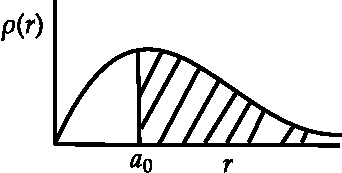
\includegraphics[height=3cm,width=5cm]{jamshi 7-crop}
		\end{figure}
	\end{minipage}
	The correct option is \textbf{(b)}
\end{answer}
\end{enumerate}



\newpage
\begin{abox}
	Practice set 2 solutions
	\end{abox}
\begin{enumerate}
	\begin{minipage}{\textwidth}
		\item The normalized ground state wavefunciton of a hydrogen atom is given by $\psi(r)=\frac{1}{\sqrt{4 \pi}} \frac{2}{a^{3 / 2}} e^{-r / a}$, where $a$ is the Bohr radius and $r$ is the distance of the electron from the nucleus, located at the origin. The expectation value $\left\langle\frac{1}{r^{2}}\right\rangle$ is
		\exyear{GATE 2011}
	\end{minipage}
	\begin{tasks}(2)
		\task[\textbf{A.}] $\frac{8 \pi}{a^{2}}$
		\task[\textbf{B.}]$\frac{4 \pi}{a^{2}}$
		\task[\textbf{C.}]$\frac{4}{a^{2}}$
		\task[\textbf{D.}]$\frac{2}{a^{2}}$
	\end{tasks}
	\begin{answer}
		$\left\langle\frac{1}{r^{2}}\right\rangle=\frac{4}{4 \pi a^{3}} \int_{0}^{\infty} \frac{1}{r^{2}} r^{2} e^{-\frac{2 r}{a}} d r \int_{0}^{\pi} \int_{0}^{2 \pi} \sin \theta d \theta d \phi=\frac{2}{a^{2}}$\\
		THe correct option is \textbf{(d)}
	\end{answer}
	\begin{minipage}{\textwidth}
		\item The ground state wavefunction for the hydrogen atom is given by $\psi_{100}=\frac{1}{\sqrt{4 \pi}}\left(\frac{1}{a_{0}}\right)^{3 / 2} e^{-r / a_{0}}$, where $a_{0}$ is the Bohr radius. The plot of the radial probability density, $P(r)$ for the hydrogen atom in the ground state is
		\exyear{GATE 2012}
	\end{minipage}
	\begin{tasks}(2)
		\task[\textbf{A.}]\begin{figure}[H]
			\centering
			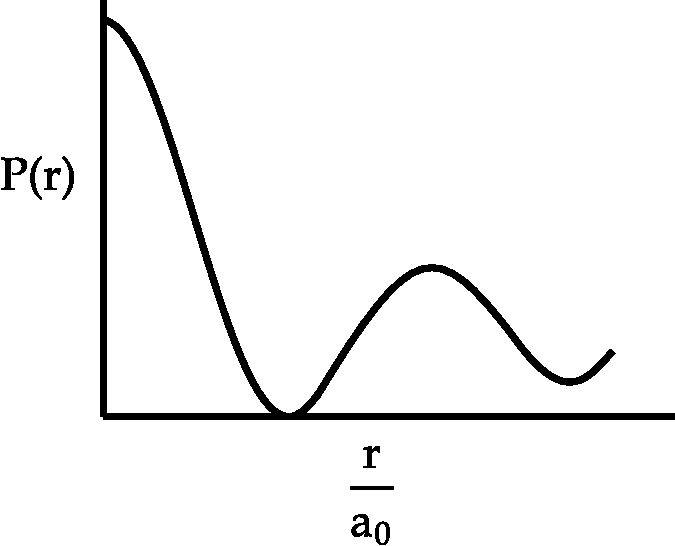
\includegraphics[height=3cm,width=5cm]{diagram-20210824(2)-crop}
			
		\end{figure}
		\task[\textbf{B.}]\begin{figure}[H]
			\centering
			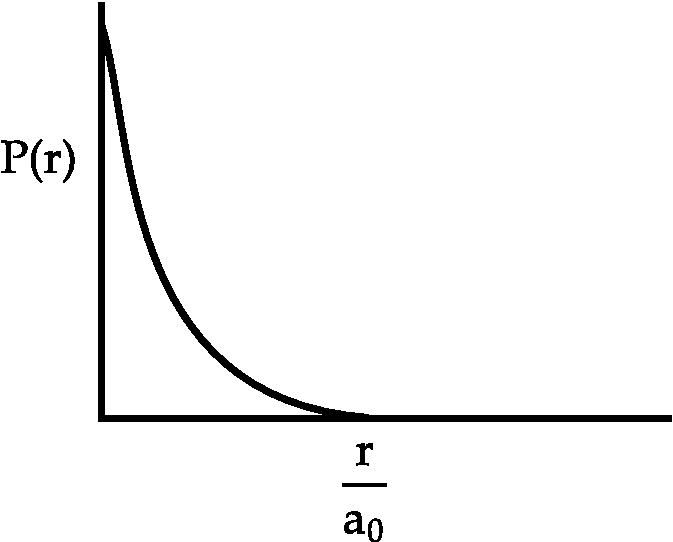
\includegraphics[height=3cm,width=5cm]{diagram-20210824(3)-crop}
			
		\end{figure}
		\task[\textbf{C.}]\begin{figure}[H]
			\centering
			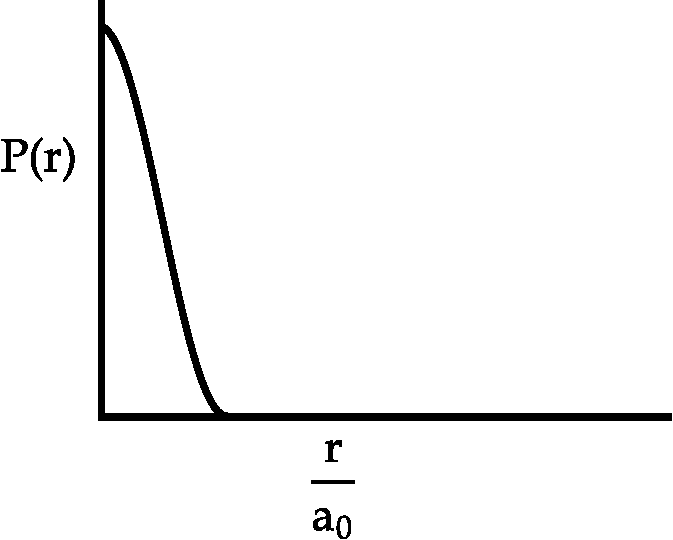
\includegraphics[height=3cm,width=5cm]{diagram-20210824(4)-crop}
			
		\end{figure}
		\task[\textbf{D.}]\begin{figure}[H]
			\centering
			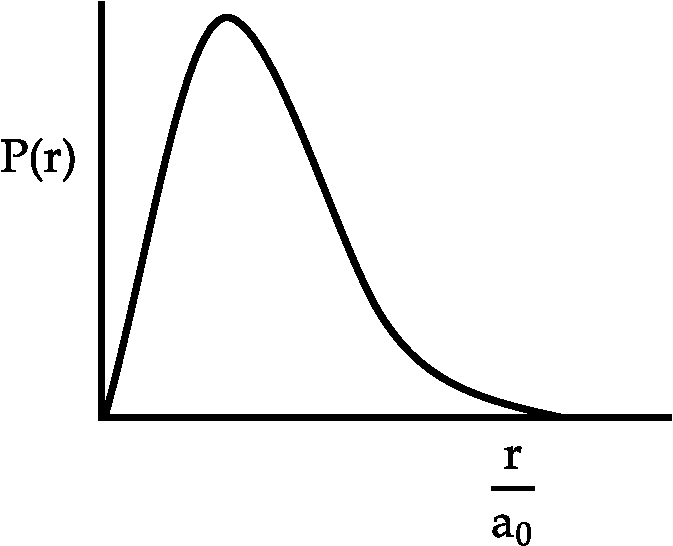
\includegraphics[height=3cm,width=5cm]{diagram-20210824(5)-crop}
		\end{figure}
	\end{tasks}
	\begin{answer}
		$\mathrm{n}$ : The ground state is given by $\psi_{100}=\frac{1}{\sqrt{4 \pi}}\left(\frac{1}{a_{0}}\right)^{3 / 2} e^{-r / a_{0}}$ Radial probability function $P(r)=|\psi|^{2} r^{2}=\frac{1}{4 \pi} \frac{1}{a_{0}^{3}} r^{2} e^{-2 r / a_{0}}$\\
		The correct option is \textbf{(d)}
	\end{answer}
	\begin{minipage}{\textwidth}
		\item An electron in the ground state of the hydrogen atom has the wave function $\psi(\vec{r})=\frac{1}{\sqrt{\pi a_{0}^{3}}} e^{-\left(\frac{r}{a_{0}}\right)}$, where $a_{0}$ is constant. The expectation value of the operator $\hat{Q}=z^{2}-r^{2}$, where $z=r \cos \theta$ is
		(Hint: $\left.\int_{0}^{\infty} e^{-a r} r^{n} d r=\frac{\sqrt{n}}{a^{n+1}}=\frac{(n-1) !}{a^{n+1}}\right)$
		\exyear{GATE 2014}
	\end{minipage}
	\begin{tasks}(2)
		\task[\textbf{A.}] $\frac{-a_{0}^{2}}{2}$
		\task[\textbf{B.}]$-a_{0}^{2}$
		\task[\textbf{C.}]$\frac{-3 a_{0}^{2}}{2}$
		\task[\textbf{D.}]$-2 a_{0}^{2}$
	\end{tasks}
	\begin{answer}
		$$\langle\hat{Q}\rangle=\left\langle z^{2}\right\rangle-\left\langle r^{2}\right\rangle \Rightarrow a_{0}^{2}-3 a_{0}^{2}=-2 a_{0}^{2}$$	
	\end{answer}
	\begin{minipage}{\textwidth}
		\item A hydrogen atom is in the state
		$$
		\psi=\sqrt{\frac{8}{21}} \psi_{200}-\sqrt{\frac{3}{7}} \psi_{310}+\sqrt{\frac{4}{21}} \psi_{321},
		$$
		where $n, l, m$ in $\psi_{n l m}$ denote the principal, orbital and magnetic quantum numbers, respectively. If $\vec{L}$ is the angular momentum operator, then the average value of $L^{2}$ is $\cdots \quad \hbar^{2}$
		\exyear{GATE 2014}
	\end{minipage}
	\begin{answer}
		If $L^{2}$ will measure on state $\psi$ the measurement is $0 \hbar^{2}, 2 \hbar^{2}$ and $6 \hbar^{2}$ with probability
		$$
		\frac{8}{21}, \frac{3}{7}, \frac{4}{21} \text { so },\left\langle L^{2}\right\rangle=2 \hbar^{2} \times \frac{3}{7}+6 \hbar^{2} \times \frac{4}{21}=2 \hbar^{2}
		$$
	\end{answer}
	\begin{minipage}{\textwidth}
		\item An electric field $\vec{E}=E_{0} \hat{z}$ is applied to a Hydrogen atom in $n=2$ excited state. Ignoring spin the $n=2$ state is fourfold degenerate, which in the $|l, m\rangle$ basis are given by $|0,0\rangle,|1,1\rangle,|1,0\rangle$ and $|1,-1\rangle$. If $H^{\prime}$ is the interaction Hamiltonian corresponding to the applied electric field, which of the following matrix elements is nonzero?
		\exyear{GATE 2019}
	\end{minipage}
	\begin{tasks}(2)
		\task[\textbf{A.}] $\left\langle 0,0\left|H^{\prime}\right| 0,0\right\rangle$
		\task[\textbf{B.}] $\left\langle 0,0\left|H^{\prime}\right| 1,1\right\rangle$
		\task[\textbf{C.}]$\left\langle 0,0\left|H^{\prime}\right| 1,0\right\rangle$
		\task[\textbf{D.}] $\left\langle 0,0\left|H^{\prime}\right| 1,-1\right\rangle$
	\end{tasks}
	\begin{answer}
		The correct option is \textbf{(c)}
	\end{answer}
\end{enumerate}
